
\begin{figure}[htbp]
    \centering
    \subfloat[Horizon $T = 3$]{
        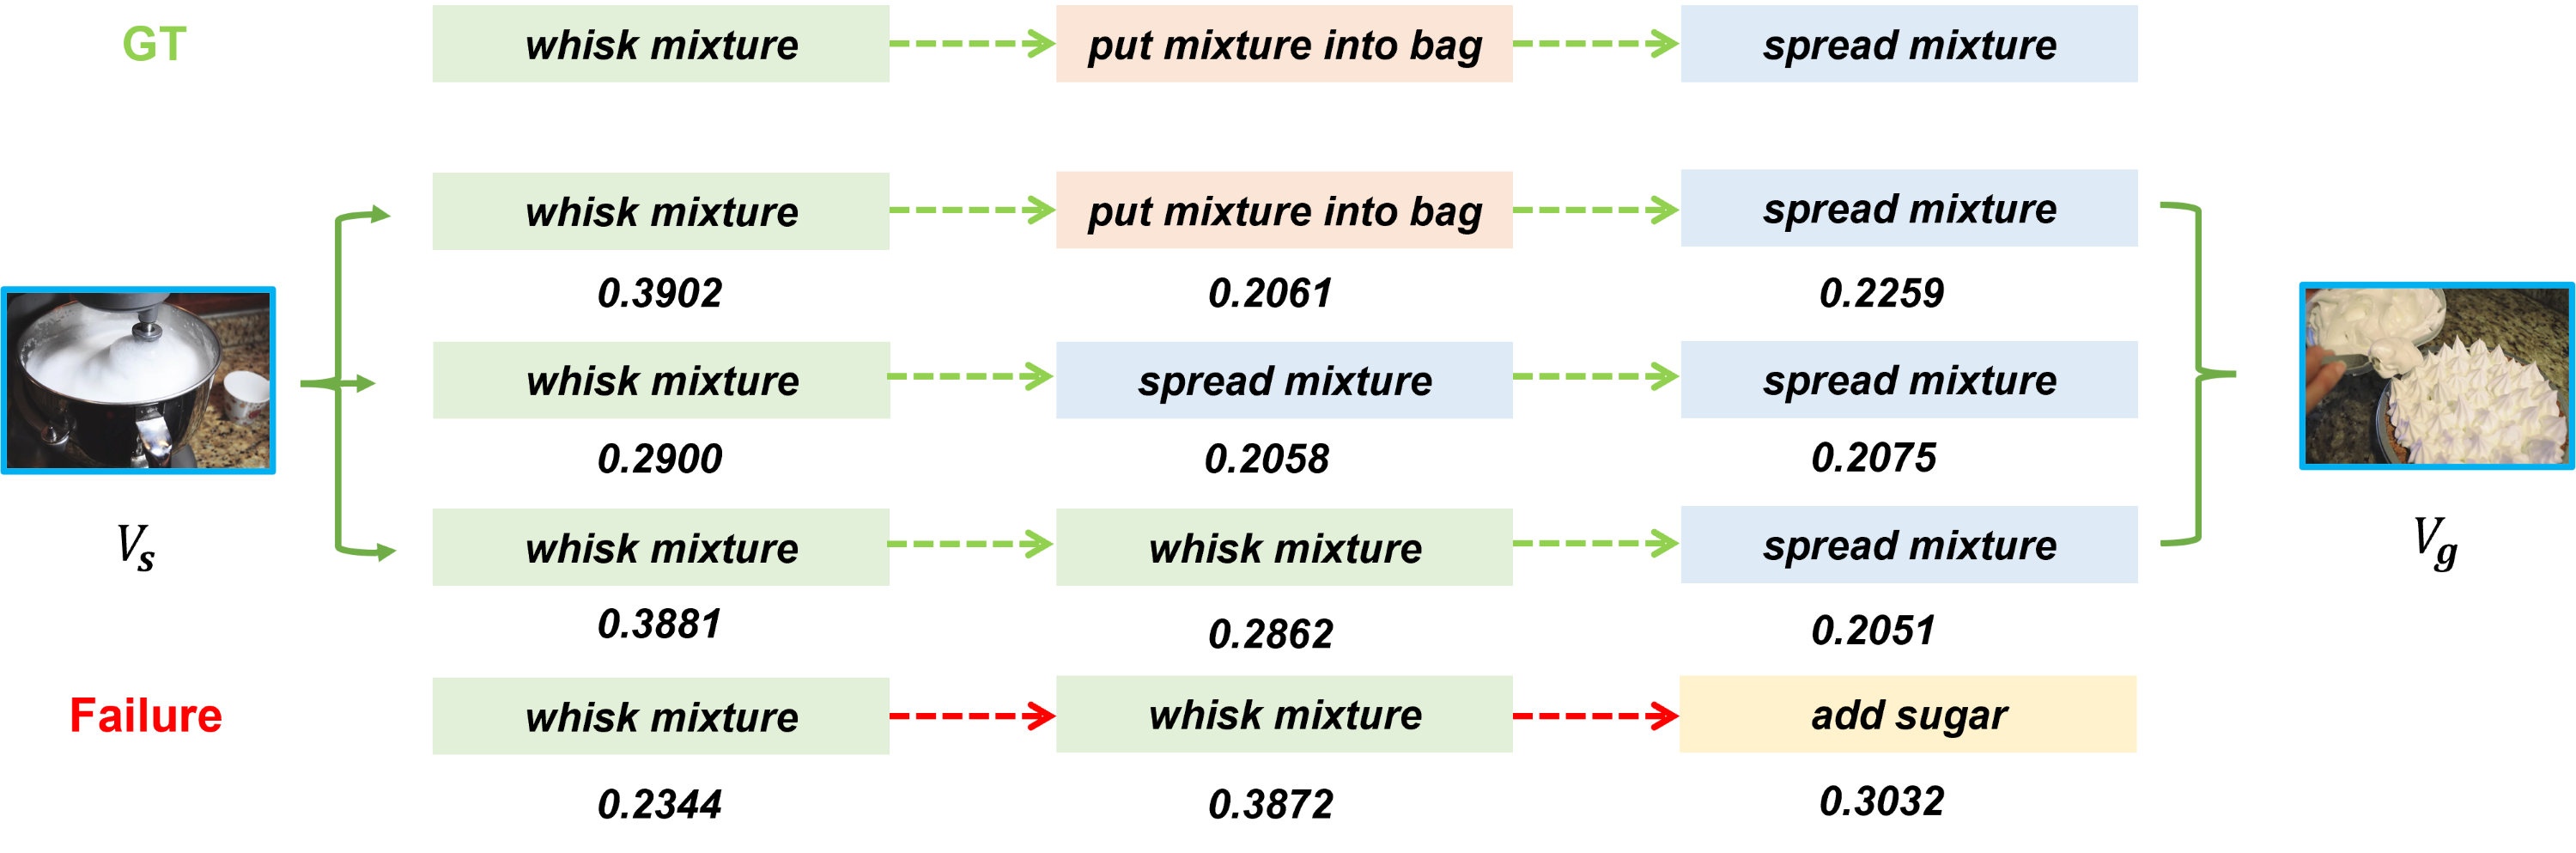
\includegraphics[width=0.95\textwidth]{figures/visualization_3.png}
        \label{fig:visual-3}
    }
    
    \vspace{1em}
    
    \subfloat[Horizon $T = 4$]{
        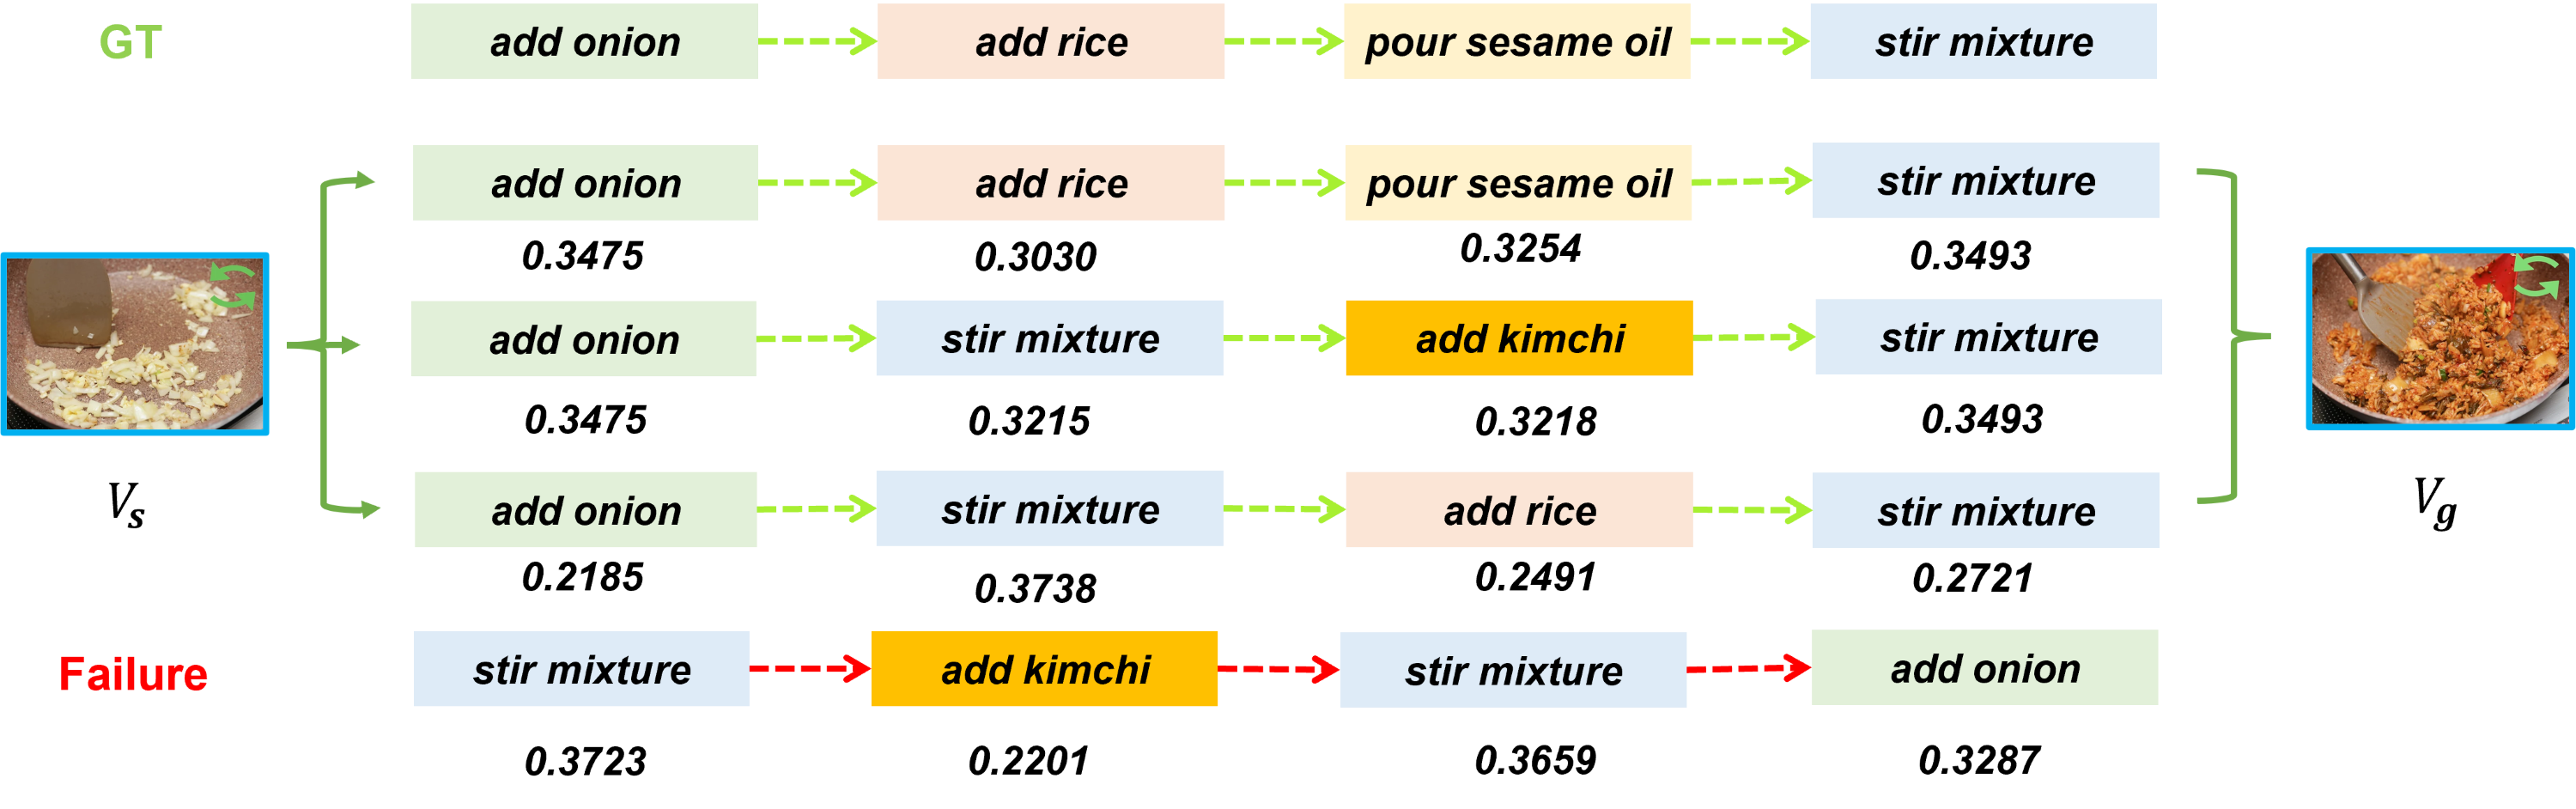
\includegraphics[width=0.95\textwidth]{figures/visualization_4.png}
        \label{fig:visual-4}
    }
    
    \vspace{1em}
    
    \subfloat[Horizon $T = 5$]{
        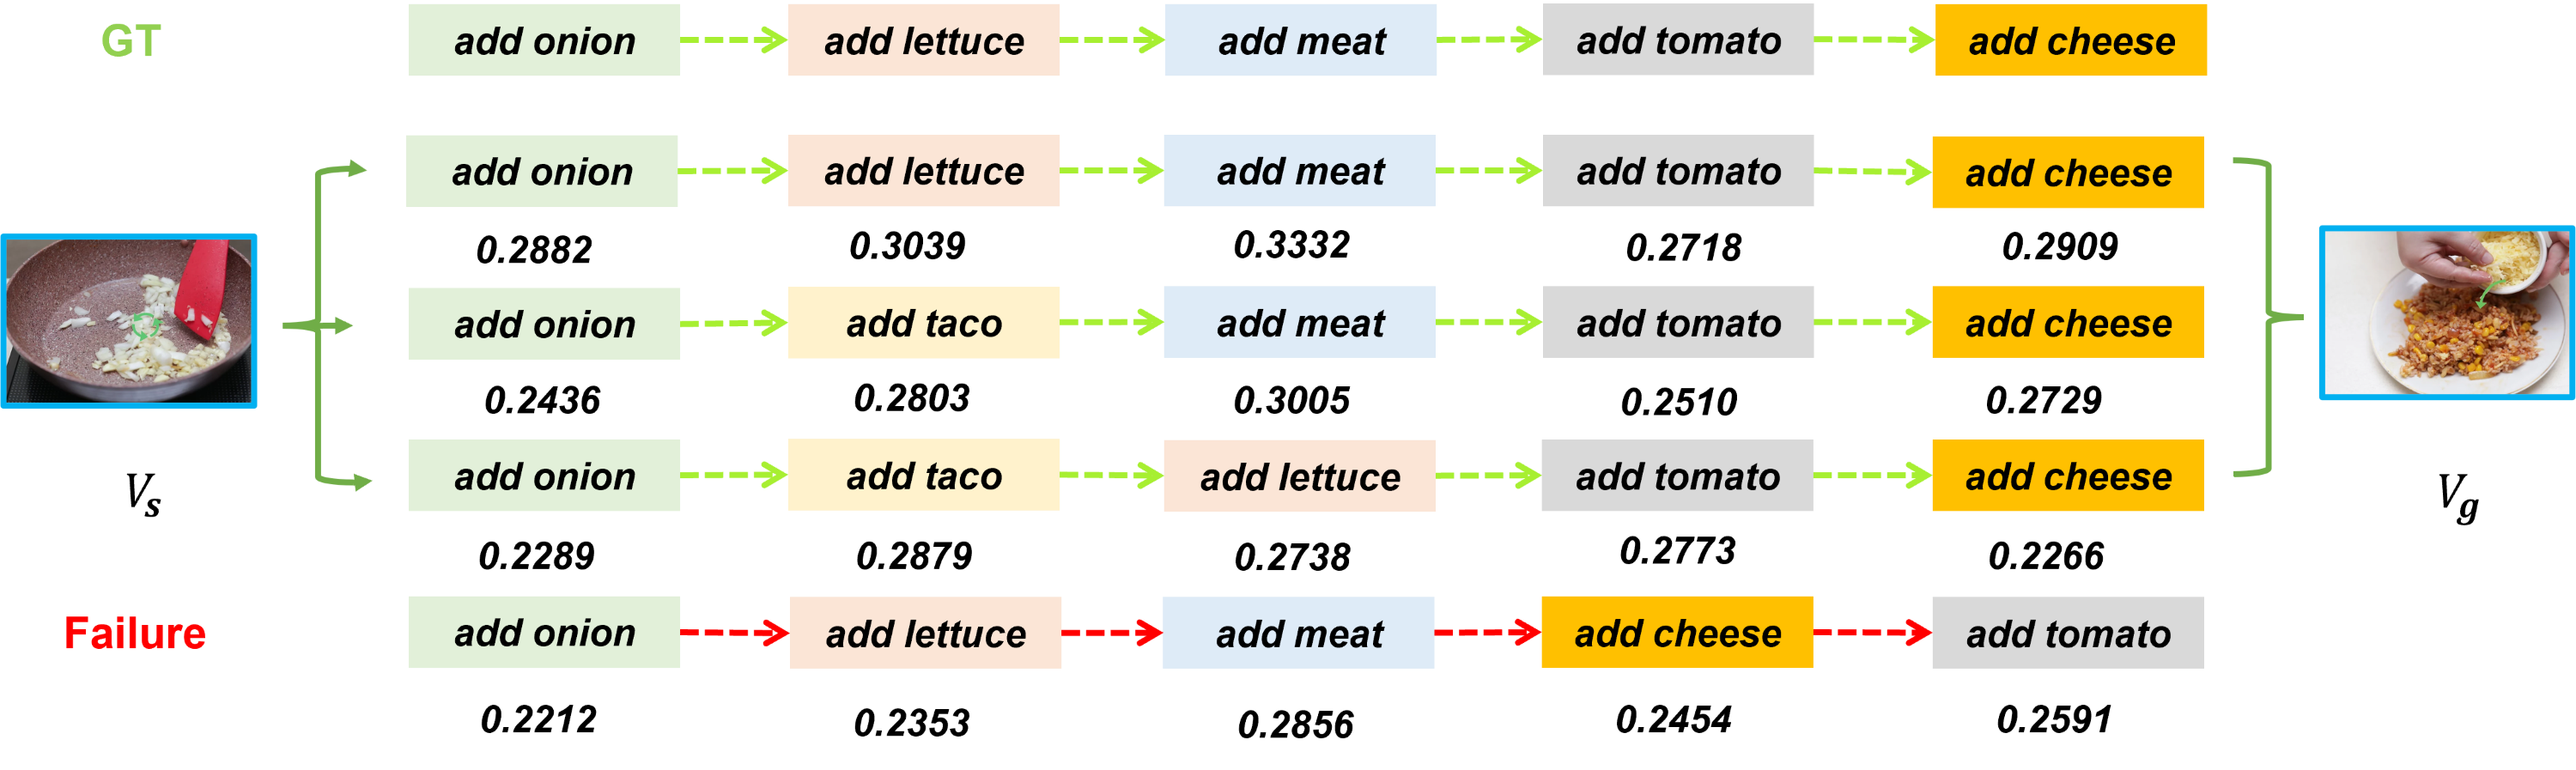
\includegraphics[width=0.95\textwidth]{figures/visualization_5.png}
        \label{fig:visual-5}
    }
    
    \vspace{1em}
    
    \subfloat[Horizon $T = 6$]{
        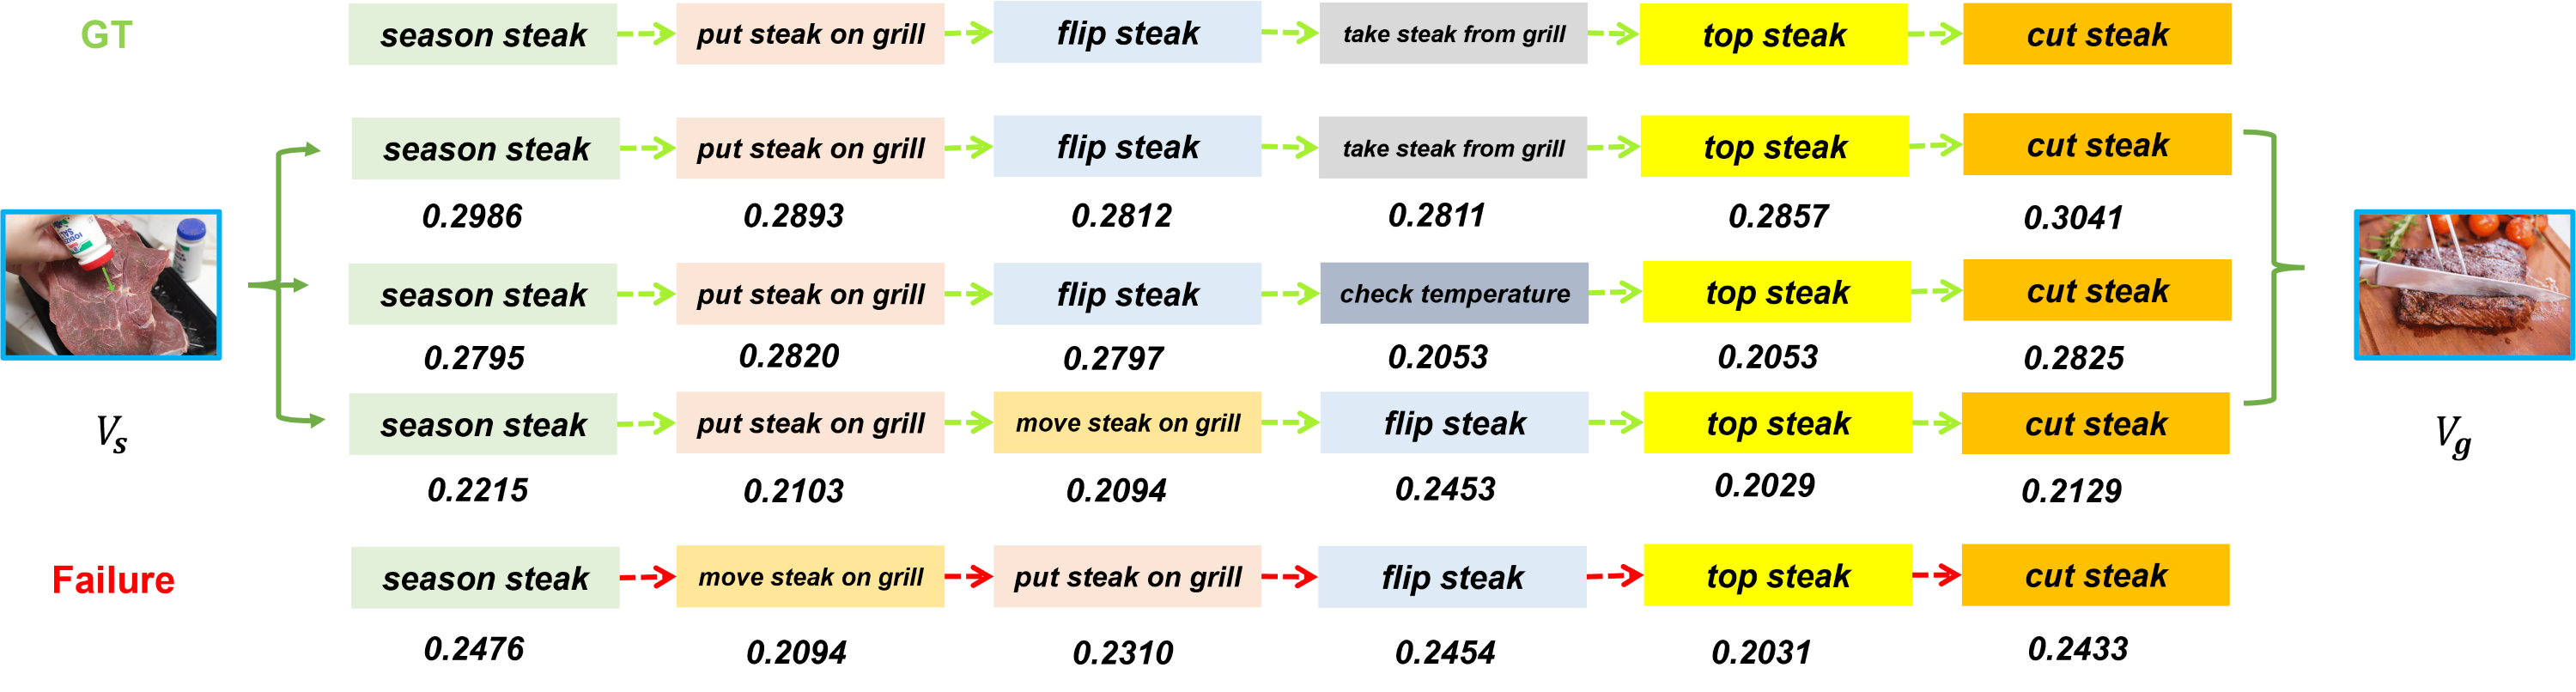
\includegraphics[width=0.95\textwidth]{figures/visualization_6.png}
        \label{fig:visual-6}
    }
    
    \caption{Visualization of diverse plans produced by our model with different horizons. Note: each figure includes images depicting the start and goal observations, the first row labeled ``GT'' showing the ground truth actions, the last row labeled ``Failure'' illustrating a plan that does not achieve the goal, and the middle rows displaying multiple reasonable plans produced by our model. These decimals represent the probability values obtained from action prediction. }
    \label{fig:visual-all}
\end{figure}